
\chapter{Wykorzystywane zagadnienia metody elementów skończonych}
\label{cha:MES_chapter}
Metoda elementów skończonych jest zaawansowanym sposobem rozwiązywania równań różniczkowych cząstkowych. Jest ona szczególnym przypadkiem metody Galerkina. Nazwa pochodzi od nazwiska Borisa Grigorievicha Galerkina, który jako pierwszy przeprowadził usystematyzowane studia na temat tego typu metod. Za pomocą tej metody można rozwiązać skomplikowane zadania dziedzin takich jak mechanika ciała stałego, mechanika płynów czy teoria pola elektromagnetycznego. Podstawy tej metody opisane są w \textcolor{red}{WieslawSrodka} oraz \textcolor{red}{Gavin}. Informacje na temat pochodzenia i estymacji błędów zaczerpnięto z \textcolor{red}{JonPointer} oraz \textcolor{red}{ErkeWand}.



\section{Rozwiązywanie zadań z  pomocą MES}
\label{sec:rozwiazwyanie_zadan}

W wytrzymałości materiałów poszukujemy zwykle sił działających w poporach konstrukcji i naprężeń wewnątrz jej konkretnych elementów. Innym podejciem jest znalezienie pola przemieszczeń dla każdego punktu konstrukcji.  W jednym i drugim przypadku znalezienie niewiadomych jest osiągalne wyłącznie dla mało skomplikowanych konstrukcji.

Metoda elementów skończonych bierze swoją nazwę od wydzielanych fragmentów konstrukcji, które są właśnie elementami skończonymi. Elementy tworzymy na siatce węzłów, które są punktami wewnątrz lub na brzegach konstrukji. Węzły są także punktami wspólnymi sąsiadujących elementów. Rozwiązanie opiera się na znalezieniu przemieszczenia węzłów i na tej podstawie obliczenia rozwiązania we wszystkich punktach wewnątrz elementów. Kolejne etapy rozwiązywania zadania za pomocą MES przedstawione są poniżej. Rysnuek \ref{fig:MES_przyklad} przedstawia przykład obiektu, który został zdyskretyzowany za pomocą elementów skończonych.

\vspace{5 mm}

\begin{enumerate}
  \item Generacja siatki węzłów.
  \item Budowa elementów skończonych na stworzonej siatce.
  \item Wyznaczanie macierzy mas i sztywności dla każdego elementu (macierze lokalne).
  \item Agregacja macierzy mas  i sztywności dla całej konstrukcji (macierze globalne).
  \item Wprowadzenie wektora obciążeń.
  \item Wprowadzenie warunków brzegowych. Mogą to być siły czynne (modyfikacja wektora obciążeń), naprężenia początkowe czy przemieszczenia wskazanych węzłów.
  \item Rozwiązanie wyznaczonego liniowego równania różniczkowego \( M \ddot x + Kx = F \) - znalezienie przemieszczeń węzłów.
  \item Wyznacznie odkształceń i naprężeń.
  \item Wyznaczenie reakcji w podporach (węzłach, dla których założono przemieszczenie)
\end{enumerate}

\vspace{5 mm}

\begin{figure}[h]
\centering
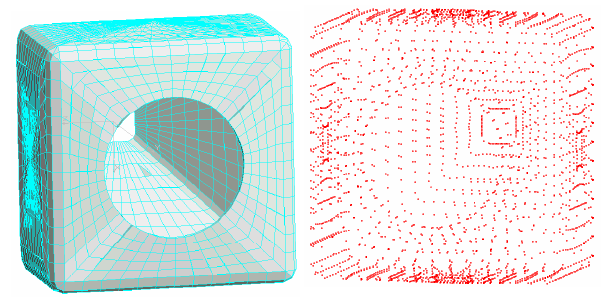
\includegraphics[width=10cm]{Zdjecia/3/MES_przyklad}
\caption{Przykład dsykretyzacji obiektu za pomocą elementów skończonych}
\label{fig:MES_przyklad}
\end{figure}

























\section{Funkcje kształtu}
\label{sec:funkcje_ksztaltu}

Weźmy metalowy pręt o długości L. W punkcie \(x_1\) na pręcie przykładamy temperaturę \( T_1 \), a w punkcie \(x_2\) temperaturę \( T_2 \). Przewidujemy, że po nieskończenie długim czasie rozkład temperatury w pręcie pomiędzy tymi punktami będzie liniowy (Rys. \ref{fig:temperatura_pret}).

\begin{figure}[h]
\centering
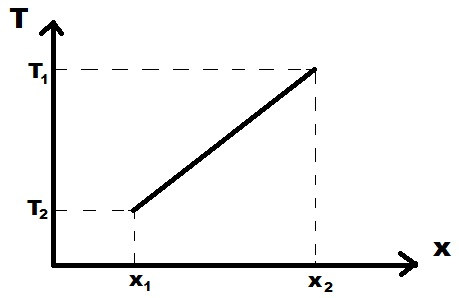
\includegraphics[width=10cm]{Zdjecia/3/rozklad_temperatury}
\caption{Temperatur pomiędzy punktami pręta}
\label{fig:temperatura_pret}
\end{figure}

Temperaturę pomiędzy tymi punktami możemy przedstawić funkcją \ref{eq:funkcja_liniowa}.

\begin{equation} \label{eq:funkcja_liniowa}
T(x)=a_0 + a_1 x, \quad dla \quad x \epsilon [x_1, x_2]
\end{equation}

Można wyznaczyć współczynniki funkcji liniowej mając dwa jej punty.

\begin{equation}
a_1 = \frac{T_2 - T_1}{x_2 - x_1}
\end{equation}

\begin{equation}
a_0 = T_2 - a_1 x_2
\end{equation}

Podstawiając współczyyniki do funkcji, możemy wyznaczyc funkcje kształtu.

\begin{equation}
T(x) = T_1 - \frac{T_2 - T_1}{L} x_1 + \frac{T_2 - T_1}{L} x = \frac{x_2 - x}{L}T_1 + \frac{x - x_1}{L}T_2 = N_1(x)T_1 + N_2(x)T_2
\end{equation}

gdzie
\begin{eqwhere}[2cm]
	\item[$N_1, N_2 $] funkcje kształtu.

\end{eqwhere}

Funkcje kształtu określają w jakim stopniu wartość temperatury z jednego węzła wpływa na wartość temperatury w dowolnym punkcie wewnątrz elementu. Dla większej liczby węzłów w jednowymiarowym elemencie funkcje kształtu są wielomianami wyższych rzędów. Poniżej znajduje się sposób wyznaczania funkcji kształtu na przykładzie 3-węzłowego elementu jednowymiarowego.

\begin{gather} \label{eq:interpolacja}
T(x) = a_0 + a_1 x + a_2 x^2 =
	\begin{bmatrix} 
	 	1 & x& x^2 \\
	\end{bmatrix}
	\begin{bmatrix} 
	 	a_0 \\
		a_1 \\
		a_2 \\
	\end{bmatrix} = \textbf{p} \textbf{a}^e = \textbf{N} \textbf{T}^e
\end{gather}

gdzie
\begin{eqwhere}[2cm]
	\item[$\textbf{p} $] wektor zmiennych kolejnych jednomianów T(x)
	\item[$\textbf{a}^e $] wektor współczynników kolejnych jednomianów T(x)
	\item[$\textbf{N} $] wektor funkcji kształtu
	\item[$\textbf{T}^e $] wektor wartości w węzłach.
\end{eqwhere}

Prawdziwe jest też poniższe równanie.

\begin{gather}
\textbf{T}^e =
	\begin{bmatrix} 
	 	1 & x_1& x_1^2 \\
		1 & x_2& x_2^2 \\
		1 & x_3& x_3^2 \\
	\end{bmatrix}
	\begin{bmatrix} 
	 	a_0 \\
		a_1 \\
		a_2 \\
	\end{bmatrix}
= \textbf{M}^e \textbf{a}^e
\end{gather}

Wyznaczając z tego równania \( \textbf{ a}^e  \) i podstawiając do równania \ref{eq:interpolacja}, otrzymamy następującą zależność.

\begin{equation}
\textbf{p a}^e = \textbf{p} {(\textbf{M}^e)}^{-1} \textbf{T}^e  = \textbf{N T}^e   \quad \Rightarrow \quad \textbf{N} = \textbf{p} {(\textbf{M}^e)}^{-1}
\end{equation}

Funkcje kształtu obliczone w taki sposób mają postać jak poniżej.

\begin{equation}
\begin{aligned}
N_1 = \frac{1}{det\textbf{M}^e} \big(x_2 x_3^2 - x_2^2 x_3 + (x_2^2 - x_3^2)x + (-x_2 + x_3)x^2\big) \\
N_2 = \frac{1}{det\textbf{M}^e} \big(x_1^2 x_3 - x_1 x_3^2 + (x_3^2 - x_1^2)x + (x_1 - x_3)x^2\big) \\
N_3 = \frac{1}{det\textbf{M}^e} \big(x_1 x_2^2 - x_1^2 x_2 + (x_1^2 - x_2^2)x + (-x_1 + x_2)x^2\big)
\end{aligned}
\end{equation}

Prawidłowo wyznaczone funkcje kształtu mają dwi ważną własności. Pierwsza związana jest z węzłami i mówi że każda funkcja przyjmuje wartość 1 w jednym węźle, a we wszystkich pozostałych 0. Druga własność mówi, że suma funkcji kształtu wewnątrz elmentu skończonego wynosi 1. Matematycznie zapisać te własności można następująco:

 \begin{equation} \label{eq:eq_zgodnosc}
	\left\{
                \begin{array}{ll}
		N_n(x_m, y_m) = 1, \quad dla \quad n=m \\
		N_n(x_m, y_m) = 0, \quad dla \quad \neq m 
                \end{array}
	\right.
 \end{equation}

 \begin{equation} \label{eq:WBS}
	\sum_1^n N_n = 1.
 \end{equation}
























\section{Wyznaczanie macierzy sztywności i mas elementów}
\label{sec:wyznaczanie_macierzy}

Weźmy model jednorodnego pręta, obciążonego jak na rysunku \ref{fig:pret} o module Younga \( E \), polu przekroju \( A \) i długości \( L \).

\begin{figure}[h]
\centering
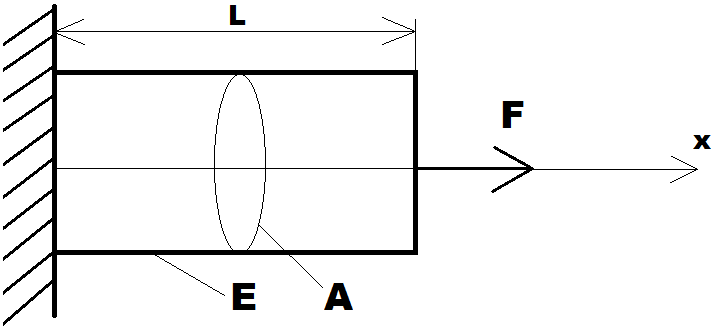
\includegraphics[width=10cm]{Zdjecia/3/pret}
\caption{Model pręta}
\label{fig:pret}
\end{figure}

Energię potencjalną i kinetyczną układu można wyrazić poniższymi wzorami.

\begin{gather} \label{eq:energia}
V = \frac{1}{2} \int_0^L \varepsilon A \sigma dx - Fu_{x=L} = \frac{1}{2} \int_0^L EA {\bigg( \frac{du}{dx}\bigg)}^2 dx - Fu_{x=L} \\
K = \frac{1}{2} \int_0^L \rho A {\bigg(\frac{\partial u}{\partial t}\bigg)}^2 dx
\end{gather}

gdzie
\begin{eqwhere}[2cm]
	\item[$V $] energia potencjalna
	\item[$K $] energia kinetyczna
	\item[$u $] przemieszczenie
	\item[$\varepsilon $] odkształcenie
	\item[$\sigma $] naprężenie
	\item[$F $] siła zewnętrzna skupiona
\end{eqwhere}
	
	Następnie stwórzmy uproszczony model, do którego wyznaczymy zależności MES.

\begin{figure}[h]
\centering
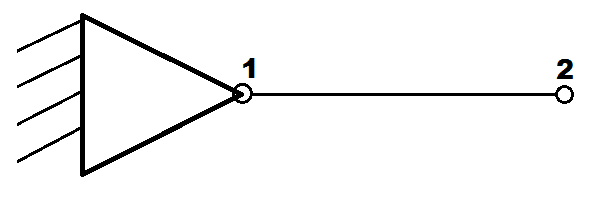
\includegraphics[width=10cm]{Zdjecia/3/pret_upr}
\caption{Uproszczony model pręta}
\label{fig:pret_upr}
\end{figure}

Znając funkcje kształtu i wartości przemieszczeń węzłów można wyznaczyć przemieszczenie w każdym punkcie pręta, a następnie odpowiednie pochodne po przemieszczeniach i po czasie.

\begin{gather}
u = N_1 x_1 + N_2 x_2 = 
	\begin{bmatrix} 
	 	N_1 & N_2 \\
	\end{bmatrix}
	\begin{bmatrix} 
	 	u_1 \\
		u_2 \\
	\end{bmatrix}
\end{gather}

\begin{gather}
\frac{\partial u}{\partial x}= 
	\begin{bmatrix} 
	 	\frac{d N_1}{d x} & \frac{d N_2}{d x} \\
	\end{bmatrix}
	\begin{bmatrix} 
	 	u_1 \\
		u_2 \\
	\end{bmatrix} = \textbf{B u}^e
\end{gather}


\begin{gather}
\frac{\partial u}{\partial t}= 
	\begin{bmatrix} 
	 	N_1 &  N_2 & \\
	\end{bmatrix}
	\begin{bmatrix} 
	 	\frac{du_1}{dt} \\
		\frac{du_2}{dt}\\
	\end{bmatrix} = \textbf{N} \dot{\textbf{u}}^e
\end{gather}


	Mając wyznaczoną energię, możemy obliczyć lagranżjan i wstawić go do dynamicznych równań Lagrangea drugiego rodzaju. Dzięki tej operacji otrzymamy końcowe, dynamiczne równanie ruchu oraz postać macierzy mas i sztywności. Równania Lagrangea drugiego rodzaju mają postać:

\begin{equation}
\frac{d}{dt} \frac{\partial L}{\partial \dot{\textbf{u}}^e} - \frac{\partial L}{\partial \textbf{u}^e} = 0, \quad L = K - V
\end{equation}

gdzie
\begin{eqwhere}[2cm]
	\item[$L$] lagranżjan.
\end{eqwhere}

Pierwszy człon wynosi

\begin{equation}
\frac{d}{dt} \frac{\partial L}{\partial \dot{\textbf{u}}^e} = \int_0^L \rho A {\textbf{N}}^T \textbf{N} {\ddot{\textbf{u}}}^e dx,
\end{equation}

zaś drugi

\begin{equation}
 \frac{\partial L}{\partial \textbf{u}^e} = -\int_0^L EA {\textbf{B}}^T \textbf{B} {\textbf{u}}^e dx + F \textbf{Nu}^e_{x=L}.
\end{equation}

Równanie dynamiki układu zapisane jest poniżej.

\begin{equation}
\int_0^L \rho A {\textbf{N}}^T \textbf{N} dx {\ddot{\textbf{u}}}^e + \int_0^L A {\textbf{B}}^T E \textbf{B} dx u = F \textbf{Nu}^e_{x=L}
\end{equation}

Postaci macierzy mas i sztywności są następujące:

\begin{gather}
\textbf{M}^e = \int_0^L \rho A {\textbf{N}}^T \textbf{N} dx \\
\textbf{K}^e = \int_0^L A {\textbf{B}}^T E \textbf{B} dx.
\end{gather}

W przypadku kiedy występuje więcej niż jedna stała materiałowa, zamiast \( E \) pojawia się macierz materiałowa \( D \). W przypadku bardziej złożonych obiektów o większej liczbie elementów skończonych, całkowanie niezbędne do obliczenia macierzy staje się bardzo czasochłonne. Ponieważ funkcje kształtu są wielomianami, optymalnym rozwiązaniem jest zastosowanie kwadratur Gaussa. Kolejny problem to określenie granic całkowania. W przypadku przedstawionym powyżej nie widać specjalnej trudności, natomiast dla trójwymiarowych obiektów o nieregularnych kształtach wymaga to dodatkowej serii obliczeń.

W takich przypadkach można zastosować mapowanie na współrzędne naturalne. W takich współrzędnych element ma z góry ustalone współrzędne węzłów, co za tym idzie także granice całkowania są znane. Dla obiektu trójwymiarowego przyjmijmy współrzędne rzeczywiste \( x, y, z \) i współrzędne naturalne \( \xi, \eta, \zeta \). Mapowania z jednych współrzędnych na drugie oblicza się według poniższego wzoru. Wizualizacja procedury przedstawiona jest na rysunku \ref{fig:izoparam}.


\begin{gather}
	\begin{bmatrix} 
	 	x \\
		y \\
		z 
	\end{bmatrix} = \sum_{i=1}^n
	\begin{bmatrix} 
	 	x_i \\
		y_i \\
		z_i 
	\end{bmatrix} N_i(\xi, \eta, \zeta)
\end{gather}

\begin{eqwhere}[2cm]
	\item[$x_i, y_i, z_i$] współrzędne rzeczywiste punktów
	\item[$N_i$] funkcje kształtu we współrzędnych naturalnych
	\item[$n$] liczba węzłów elementu.
\end{eqwhere}

\begin{figure}[h]
\centering
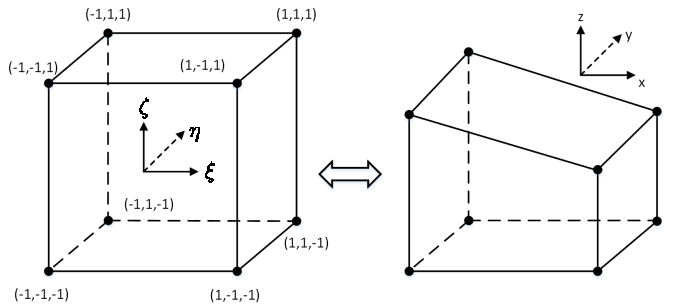
\includegraphics[width=10cm]{Zdjecia/3/izoparam}
\caption{Przekształcenie izoparametryczne}
\label{fig:izoparam}
\end{figure}

Dla elementów w takich współrzędnych funkcje kształtu są znane i stabelaryzowane. Dla elementu sześciennego wypisane są w \ref{eq:f_ksztaltu_hex}.

\begin{equation} \label{eq:f_ksztaltu_hex}
	\begin{aligned}
		N_1 = \frac{1}{8}(1-\xi)(1-\eta)(1-\zeta) \\
		N_2 = \frac{1}{8}(1+\xi)(1-\eta)(1-\zeta) \\
		N_3 = \frac{1}{8}(1+\xi)(1+\eta)(1-\zeta) \\
		N_4 = \frac{1}{8}(1-\xi)(1+\eta)(1-\zeta) \\
		N_5 = \frac{1}{8}(1-\xi)(1-\eta)(1+\zeta) \\
		N_6 = \frac{1}{8}(1+\xi)(1-\eta)(1+\zeta) \\
		N_7 = \frac{1}{8}(1+\xi)(1+\eta)(1+\zeta) \\
		N_8 = \frac{1}{8}(1-\xi)(1+\eta)(1+\zeta)
	\end{aligned}
\end{equation}

Ostatnim elmentem niezbędnym do prawidłowego całkowania we współrzędnych naturalnych jest wyznaczenie jakobianu przekształcenia. Macierz Jacobiego przedstawiona jest w równaniu \ref{eq:m_jacobiego}.

\begin{gather} \label{eq:m_jacobiego}
	\textbf{J} = \begin{bmatrix} 
	 	\frac{\partial x}{\partial \xi} & \frac{\partial y}{\partial \xi} & \frac{\partial z}{\partial \xi} \\
	 	\frac{\partial x}{\partial \eta} & \frac{\partial y}{\partial \eta} & \frac{\partial z}{\partial \eta} \\
	 	\frac{\partial x}{\partial \zeta} & \frac{\partial y}{\partial \zeta} & \frac{\partial z}{\partial \zeta}
	\end{bmatrix}
\end{gather}

Ostatecznie wyznaczanie macierzy mas i sztywności dla elementu sześciennego zostanie zmodyfikowane jak poniżej:

\begin{equation} \label{eq:macierz_sztywnosci}
	\begin{aligned}
	\textbf{K}^e = \int_V {\textbf{B}}^T E \textbf{B} dV \quad \rightarrow \quad \textbf{K}^e =  \int_{-1}^1 \int_{-1}^1 \int_{-1}^1  {\textbf{B}}^T \textbf{D} \textbf{B} det\textbf{J} d\xi d\eta d\zeta.
	\end{aligned}
\end{equation}

\begin{equation} \label{eq:macierz_mas}
	\begin{aligned}
	\textbf{M}^e = \int_V \rho {\textbf{N}}^T \textbf{N} dV \quad \rightarrow \quad \textbf{M}^e = \int_{-1}^1 \int_{-1}^1 \int_{-1}^1 \rho {\textbf{N}}^T \textbf{N} det\textbf{J} d\xi d\eta d\zeta \\
	\end{aligned}
\end{equation}
























\section{Agregacja globalnych macierzy mas i sztywności}
\label{sec:agregacja}

Metoda agregacji macierzy globalnych zostanie przedstawiona na przykładzie macierzy sztywności dwóch elmentów kwadrratowych i obiektu z nich zbudowanego. Wspomniany obiekt przedstawia rysunek \ref{fig:agreg}. Czarne cyfry oznaczają numerację lokalną wewnątrz elmentu, a czerwone numerację globalną.

Algorytm agregacji polega na umieszczaniu odpowiednich elementów macierzy lokalnych do macierzy globalnej. Pokrywające się elementy są sumowane. Ponieważ podmacierz sztywności dla jednego punktu lub zależności pomiędzy punktami jest umieszczana w macierzy globalnej bez wewnętrznych zmian, przyjmijmy zapis uproszczony:

\begin{figure}[h]
\centering
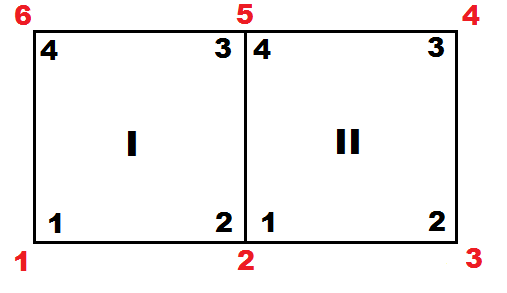
\includegraphics[width=10cm]{Zdjecia/3/agregacja}
\caption{Dwa elementy skończone kwadratowe tworzące obiekt}
\label{fig:agreg}
\end{figure}

\begin{gather}
	\textbf{K}_n^{ij} = \begin{bmatrix} 
	 	K^{ij}_{xx} & K^{ij}_{xy} \\
	 	K^{ij}_{xy} & K^{ij}_{yy} \\
	\end{bmatrix}
\end{gather}

gdzie
\begin{eqwhere}[2cm]
	\item[$i, j$] numery punktów
	\item[$n$] numer elementu
	\item[$x, y$] współrzędne punktów.
\end{eqwhere}

W takim wypadku lokalne macierze sztywności dla obydwu elementów możemy zapisać jako:

\begin{gather}
	\textbf{K}_{I} = \begin{bmatrix} 
	 	\textbf{K}^{11}_I & \textbf{K}^{12}_I & \textbf{K}^{13}_I & \textbf{K}^{14}_I \\
	 	\textbf{K}^{21}_I & \textbf{K}^{22}_I & \textbf{K}^{23}_I & \textbf{K}^{24}_I \\
	 	\textbf{K}^{31}_I & \textbf{K}^{32}_I & \textbf{K}^{33}_I & \textbf{K}^{34}_I \\
	 	\textbf{K}^{41}_I & \textbf{K}^{42}_I & \textbf{K}^{43}_I & \textbf{K}^{44}_I
	\end{bmatrix} \\
	\textbf{K}_{II} = \begin{bmatrix} 
	 	\textbf{K}^{11}_{II} & \textbf{K}^{12}_{II} & \textbf{K}^{13}_{II} & \textbf{K}^{14}_{II} \\
	 	\textbf{K}^{21}_{II} & \textbf{K}^{22}_{II} & \textbf{K}^{23}_{II} & \textbf{K}^{24}_{II} \\
	 	\textbf{K}^{31}_{II} & \textbf{K}^{32}_{II} & \textbf{K}^{33}_{II} & \textbf{K}^{34}_{II} \\
	 	\textbf{K}^{41}_{II} & \textbf{K}^{42}_{II} & \textbf{K}^{43}_{II} & \textbf{K}^{44}_{II}
	\end{bmatrix}.
\end{gather}

Macierze te mają wymiar 8x8, co odpowiada czterem punktom i dwóm współrzędnym dla każdego punktu. Macierz globalna wobec tego będzie miała wymiar 12x12 (6x6 podmacierzy). Poniżej przedstawione jest wyznaczanie kilku elmentów macierzy globalnej.

Dla globalnego punktu 1 mamy:
\begin{equation}
	\textbf{K}^{11} = \textbf{K}_I^{11},
\end{equation}
ponieważ punkt globalny 1 pokrywa się z punktem 1 macierzy I.

Dla globalnego punktu 2 mamy:
\begin{equation}
	\textbf{K}^{22} = \textbf{K}_I^{22} + \textbf{K}_{II}^{11},
\end{equation}
ponieważ punkt globalny 2 pokrywa się z punktem 2 macierzy I oraz punktem 1 macierzy II.

Dla zależności globalnych punktów 2 i 3 mamy:
\begin{equation}
	\textbf{K}^{23} = \textbf{K}_{II}^{12},
\end{equation}
ponieważ punkt globalny 2 pokrywa się z punktem 1, a punkt globalny 3 z punktem 2 macierzy II.

Dla zależności globalnych punktów 2 i 5 mamy:
\begin{equation}
	\textbf{K}^{25} = \textbf{K}_{I}^{23} + \textbf{K}_{II}^{14},
\end{equation}
ponieważ punkt globalny 2 pokrywa się z punktem 2 macierzy I oraz punktem 1 macierzy II, a punkt globalny 5 z punktem 3 macierzy I oraz punktem 4 macierzy II.

Uwzględniając że sztywność względna punktów nie będących ze sobą w sąsiedztwie (np. 1 w pierwszym elemencie oraz 3 w drugim elemencie) wynosi 0, macierz globalna przyjmuje postać:

\begin{gather}
	\textbf{K} = \begin{bmatrix} 
	 	\textbf{K}^{11}_I & \textbf{K}^{12}_I & 0 & 0 & \textbf{K}^{13}_I & \textbf{K}^{14}_I  \\
	 	\textbf{K}^{21}_I & \textbf{K}^{22}_I + \textbf{K}^{11}_{II}  & \textbf{K}^{12}_{II} & \textbf{K}^{13}_II & \textbf{K}_{I}^{23} + \textbf{K}_{II}^{14} & \textbf{K}^{24}_I \\
	 	0 & \textbf{K}^{21}_{II} & \textbf{K}^{22}_{II} & \textbf{K}^{23}_{II} & \textbf{K}^{24}_II & 0 \\
	 	0 & \textbf{K}^{31}_II & \textbf{K}^{32}_{II} & \textbf{K}^{33}_{II} & \textbf{K}^{34}_{II} & 0 \\
		\textbf{K}^{31}_I & \textbf{K}_{I}^{32} + \textbf{K}_{II}^{41} & \textbf{K}^{42}_II & \textbf{K}^{43}_{II} & \textbf{K}^{33}_{I} + \textbf{K}	^{44}_{II} & \textbf{K}^{34}_{I} \\
		\textbf{K}^{41}_I & \textbf{K}^{42}_I & 0 & 0 & \textbf{K}^{43}_I & \textbf{K}^{44}_I.
	\end{bmatrix}
\end{gather}

Oczywistym jest, że w przypadku innej numeracji węzłów globalnych zmieni się układ macierzy globalnej. Nie ma to jednak wpływu na ostateczny wynik rozwiązania MES. W modelach o dużej liczbie elmentów skończonych macierze mas i sztywności są macierzami rzadkimi. Wykorzystuje się to w obliczeniach do oszczędzania pamięci komputera, poprzez zapis w pamięci tylko wartości niezerowych oraz ich położenia w macierzy. 

Macierz mas wyznaczona w przedstawiony sposób jest nazywana macierzą konsystentną. Często stosuje się macierze skupione, które zawierają elementy tylko na diagonali. Pozwala to bardzo przyspieszyć obliczenia. Takie rozwiązanie jest ściśle rzecz biorąc niepoprawne, ponieważ nie ma algorytmu, który pozwala obliczyć macierz skupioną i zachować w pełni właściwości modelu. Macierze skupione oblicza się np. poprzez sumowanie wszystkich elmentów w wierszu i umieszczanie tej sumy na elemencie diagonalnym. Dobrą stroną macierzy skupionych jest fakt, że rozwiązanie pozostaje zbieżne.






















\section{Rozwiązanie wyznaczonego równania macierzowego}
\label{sec:rozwiazanie_r_roz}

Przyjmijmy, że wyznaczone równanie różniczkowe po agregacji macierzy ma postać:

\begin{equation} \label{eq:mes_wyjsciowe}
	\textbf{M} \ddot{\textbf{x}} + \textbf{Kx} = \textbf{F}.
\end{equation}

Rozwiązać to równanie można na wiele sposobów. Przedstawione zostaną tutaj trzy. Pierwszy sposób to metoda całkowania jawnego, druga - metoda całkowania niejawnego, a trzecie to metoda modalna.

W metodzie całkowania jawnego zakładamy rozpoczęcie obliczeń w kroku czasowym t i przybliżamy pochodną drugiego rzędu poprzez formułę centralną:

\begin{equation}
	\ddot{\textbf{x}}^t = \frac{\textbf{x}^{t+1} - 2\textbf{x}^t + \textbf{x}^{t-1}}{\delta t^2}.
\end{equation}

Po podstawieniu do równania \ref{eq:mes_wyjsciowe} wyznaczamy \( \textbf{x}^{t+1} \):

\begin{equation} \label{eq:jawne_calkowanie}
	\textbf{x}^{t+1} = \Delta t^2 \textbf{M}^{-1}(\textbf{F}^t - \textbf{Kx}^t) + 2\textbf{x}^t - \textbf{x}^{t-1}.
\end{equation}

Metoda ta charakteryzuje się tym, że do stabilności rozwiązania często wymaga małego kroku czasowego. Nadaje się ona za to do zrównoleglania obliczeń, co pozwala zastosować do tego celu procesory graficzne. Operacja odwracania macierzy \( \textbf{M} \) we wzorze \ref{eq:jawne_calkowanie} jest kosztowna obliczeniowo. Zastosowanie macierzy skupionej pozwala znacznie przyspieszyć tą procedurę.

Metoda całkowania niejawnego różni się wyjściowym krokiem czasowym. Zakładamy początkową chwilę czasową \( t+1 \), co przy zastosowaniu tej samej formuły różnicowej wprowadza krok wstecz.

\begin{equation} \label{eq:niejawne}
	\ddot{\textbf{x}}^{t+1} = \frac{\textbf{x}^{t+1} - 2\textbf{x}^t + \textbf{x}^{t-1}}{\delta t^2}.
\end{equation}

Podstawiamy równanie \ref{eq:niejawne} do równania

\begin{equation} \label{eq:mes_wyjsciowe}
	\textbf{M} \ddot{\textbf{x}}^{t+1} + \textbf{Kx}^{t+1} = \textbf{F}^{t+1}
\end{equation}

i otrzymujemy 

\begin{equation} 
	\textbf{x}^{t+1} = (\textbf{M} + \Delta t^2 \textbf{K})^{-1} (\Delta t^2 \textbf{F}^{t+1} + 2\textbf{MX}^t - \textbf{MX}^{t-1}.
\end{equation}

W tym wypadku nie unikniemy już odwracania macierzy \( \textbf{M} + \Delta t^2 \textbf{K} \), co powoduje wydłużenie obliczeń. Zaletą tej metody jest fakt, że jest ona bezwarunkowo stabilna.

W metodzie modalnej jako pierwsze należy wyznaczyć wektory własne dla równania jednorodnego \( \textbf{M} \ddot{\textbf{x}} + \textbf{Kx} = 0 \). Wektory własne wyznaczyć można z dokładnością do stałej multiplikatywnej. Możliwe jest wyskalowanie tych wektorów w taki sposób, aby maciesz tych wektorów \( \boldsymbol{\phi} \) miała własność:

\begin{equation} 
	\boldsymbol{\phi}^T \textbf{M} \boldsymbol{\phi} = \textbf{I}.
\end{equation}

Zakładając przekształcenie współrzędnych \( \textbf{x} = \boldsymbol{\phi} \overbar{\textbf{x}}  \) otrzymamy nową postać równania \ref{eq:mes_wyjsciowe}.

\begin{equation} 
	\ddot{\overbar{\textbf{x}}} + \boldsymbol{\Lambda} \overbar{\textbf{x}} = \overbar{\textbf{F}}, \quad \boldsymbol{\Lambda} = \boldsymbol{\phi}^T\textbf{K}\boldsymbol{\phi}, \quad \overbar{\textbf{F}} = \boldsymbol{\phi}^T \textbf{F}.
\end{equation}

Macierz \( \boldsymbol{\Lambda} \) jest macierzą diagonalną, więc rozwiązanie układu sprowadza się teraz do znalezienia rozwiązania dla pojedynczych oscylatorów harmonicznych. Elementy macierzy \( \boldsymbol{\Lambda} \) są kwadratami częstości własnych drgań węzłów.

\begin{gather}
	\begin{bmatrix} 
		\ddot{\overbar{x}_1} \\
		\ddot{\overbar{x}_2} \\
		\ddot{\overbar{x}_3} \\
		\vdots \\
		\ddot{\overbar{x}_n}
	\end{bmatrix} +
	\begin{bmatrix} 
		\omega_1^2	&			&			&				& \\
				& \omega_2^2	& 			& \text{\huge{0}}		& \\
				&			& \omega_3^2 	& 				& \\
				& \text{\huge{0}}	& 			& \ddots			& \\
				&			&			&				& \omega_n^2
	\end{bmatrix}
	\begin{bmatrix} 
		\overbar{x}_1 \\
		\overbar{x}_2 \\
		\overbar{x}_3 \\
		\vdots \\
		\overbar{x}_n
	\end{bmatrix} =
	\begin{bmatrix} 
		\overbar{F}_1 \\
		\overbar{F}_2 \\
		\overbar{F}_3 \\
		\vdots \\
		\overbar{F}_n
	\end{bmatrix}
\end{gather}

 \begin{equation}
	\left\{
                \begin{array}{ll}
  		\ddot{\overbar{x}_1}+\omega_1^2\overbar{x}_1=\overbar{F}_1 \quad \rightarrow\\
  		\ddot{\overbar{x}_2}+\omega_2^2\overbar{x}_2=\overbar{F}_2 \quad \rightarrow\\
  		\ddot{\overbar{x}_3}+\omega_3^2\overbar{x}_3=\overbar{F}_3 \quad \rightarrow\\
		\quad \quad \vdots \quad \quad \\
  		\ddot{\overbar{x}_n}+\omega_n^2\overbar{x}_n=\overbar{F}_n \quad \rightarrow
                \end{array}
	\begin{bmatrix} 
		\overbar{x}_1 \\
		\overbar{x}_2 \\
		\overbar{x}_3 \\
		\vdots \\
		\overbar{x}_n
	\end{bmatrix}
	\right.
 \end{equation}

Po rozwiązaniu równań należy wyznaczyć ostateczne rozwiązanie \( \textbf{x} = \boldsymbol{\phi} \overbar{\textbf{x}}  \).




















\section{Zbieżność metody i błędy rozwiązania}
\label{sec:zbieznosc_i_blad}

O zbieżności rozwiązania możemy wnioskować na podstawie funkcji kształtu. Pierwszym warunkiem jest tzw. warunek zgodności. Mówi on o tym, że funkcje kształtu muszą być ciągłe w przestrzeni elementów. Dla prostego przypadku dwóch elementów liniowych jednowymiarowych ciągłość funkcji ilustruje rysunek \ref{fig:zgodnosc}. 

\begin{figure}[h]
\centering
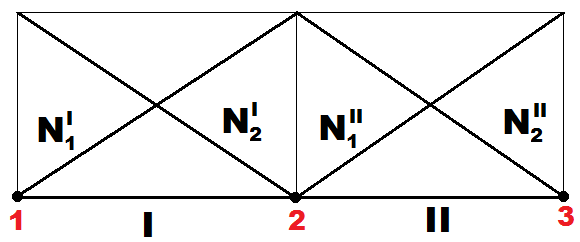
\includegraphics[width=10cm]{Zdjecia/3/zgodnosc}
\caption{Ciągłość funkcji w przestrzenii elementów}
\label{fig:zgodnosc}
\end{figure}

Warunek ten jest zapewniony poprzez własność funkcji kształtu przedstawioną we wzorze \ref{eq:eq_zgodnosc}.

Kolejny warunek nazywa się warunkiem bryły sztywnej (WBS). Zapewnia on brak straty bądź narastania energii podczas wyznaczania wyniku wewnątrz elementu. Warunek ten jest zapewniony poprzez własność funkcji kształtu przedstawioną w \ref{eq:WBS}.

Ostatnim warunkiem jest tzw. warunek stałego odkształcenia (WSO). Mówi on o tym, że jeśli w elemencie przyłożymy liniowe pole przemieszczeń, to odkształcenie będzie stałe w każdym punkcie elementu.

Jeśli spełnione są warunki zgodności, WBS oraz WBO to rozwiązanie dla elementu będzie zbieżne. Warunki te muszą być spełnione dla każdego elementu obliczanego modelu.

\vspace{3mm}

Zbieżność nie daje nam gwarancji, że rozwiązanie otrzymane przy pomocy symulacji MES jest poprawne. Przez poprawne rozumiane jest, że błąd rozwiązania jest dostatecznie mały. Aby mieć pewność, że rozwiązanie jest wystarczająco dokładne należy oszacować błąd maksymalny. W przypadku MES błąd powodują:

\begin{enumerate}
	\item dyskretyzacja konstrukcji 
	\item zaokrąglenia arytmetyczne.
\end{enumerate}

\vspace{3mm}

Pierwsza przyczyna występowania błędów związana jest z podziałem konstrukcji na elementy skończone. Błąd zawarty jest już w równaniu \( \textbf{M} \ddot{\textbf{x}} + \textbf{Kx} = \textbf{F} \). Pojawia się dlatego, że całe rozwiązanie wyznaczamy za pomocą wielomianowych funkcji kształtu. Błąd zbieżnego rozwiązania możemy zmniejszać poprzez wykorzystanie funkcji kształtu wyższego rzędu, bądź zagęszczenie siatki i budowę większej liczby elementów skończonych.

Estymacja błędów odbywa się na różne sposoby. Jednym z nich jest wykorzystanie równania \ref{eq:blad1}. 

\begin{equation} \label{eq:blad1}
	F - \tilde{F}_i \approx ch_i^r
\end{equation}

gdzie
\begin{eqwhere}[2cm]
	\item[$ F $] rozwiązanie dokładne
	\item[$ \tilde{F}_i $] i-te rozwiązanie przybliżone
	\item[$ c $] współczynnik proporcjonalności
	\item[$ h_i $] współczynnik zależny od zagęszczenia siatki
	\item[$ r $] współczynnik zależny od stopnia wielomianów interpolujących.
\end{eqwhere}

Jedna symulacja nie daje możliwości wyznaczyć błędu. Aby tego dokonać należy przeprowadzić dwie symulacje, co pozwala obliczyć błąd drugiej (dokładniejszej). Przyjmijmy, że druga symulacja zawiera elementy o dwukrotnie mniejszych wymiarach, czyli \( h_1 = 2h_2 \). Współczynnik \( r \) przyjmuje wartości mniejsze od 1, ale dla uproszczenia przyjmijmy dokładnie 1.

Podstawiając odpowiednie indeksy do wzoru \ref{eq:blad1}, możemy wyznaczyć błąd drugiej symulacji, znając wyniki zarówno pierwszej jak i drugiej.

\begin{equation} 
	F- \tilde{F}_2 \approx \frac{\tilde{F}_2 - \tilde{F}_1}{(\frac{h_1}{h_2})^r - 1}.
\end{equation}

Innym podejściem jest wyznaczanie błędów poprzez energię naprężenia elementów. Po wyznaczeniu przemieszczeń węzłów i obliczeniu naprężeń, naprężenia nie są ciągłe w przestrzeni elementów. Jeśli jeden węzeł należy do kilku elementów, to w każdym z nich może zostać wyznaczona inna wartość naprężenia dla takiego węzła. W ciągłym przypadku naprężenie byłoby funkcją ciągłą, dlatego błąd wynikający z naprężeń wyznacza się w następujący sposób:

\vspace{3mm}

\begin{enumerate}
	\item Obliczamy średnią naprężeń w węźle, biorąc wartości dla węzła z każdego elementu, do którego należy.
	\item Wyznaczamy błąd naprężenia w węzłach elementu, poprzez odejmowanie od naprężenia w węźle wartości średniego naprężenia w tym węźle.
	\item Sumujemy błędy naprężeń wszystkich elementów skończonych.
	\item Wyznaczamy energię błędu naprężenia.
	\item Wyznaczamy energię odkształcenia dla całej konstrukcji.
	\item Obliczamy błąd procentowy według wzoru \ref{eq:blad2}.
\end{enumerate}

\vspace{3mm}

\begin{equation} \label{eq:blad2}
	E = 100(\frac{e}{U + e})^{0.5}
\end{equation}

gdzie
\begin{eqwhere}[2cm]
	\item[$ e $] całkowita energi błędu dla konstrukcji
	\item[$ U $] energi odkształcenia dla konstrukcji
	\item[$ E $] błąd procentowy energii.
\end{eqwhere}











































